%versi 3 (22-07-2020)
\chapter{Landasan Teori}
\label{chap:teori}

Bab ini akan berisikan tentang beberapa teori dari metode atau hal-hal yang diperlukan dalam melakukan penelitian ini seperti apa itu \http, SQL, statistika, dan visualisasi data.

\section{\http~\cite{httpreports}}
\label{sec:httparchive} 

\http merupakan sebuah situs \web yang menyediakan catatan dari kurun waktu tertentu. Hal ini dilakukan agar pemilik halaman \web dapat melihat kembali hal yang sudah terjadi, perilaku yang sedang terjadi, dan menemukan tren yang akan muncul.

 
\subsection{\textit{Reports}}
\label{subsec:reports}

\textit{Reports} berisi informasi terperinci mengenai sumber daya yang diambil, API dan fitur platform yang digunakan, serta jejak eksekusi dari setiap halaman dari situs-situs teratas yang ada di \web. Informasi yang telah didapatkan kemudian diolah dan dianalisis untuk melihat perkembangan tren. \textit{Reports} yang dimiliki oleh situs \http dibagi menjadi beberapa kategori. Kategori tersebut adalah sebagai berikut:

\subsubsection{\textit{State of the Web}} 
\label{subsub:StateWeb}

\textit{State of the Web} berisi \textit{report} yang menangkap perkembangan \web secara jangka panjang  termasuk teknik untuk efisiensi jaringan dan penggunaan standar seperti HTTPS. \textit{Reports} ini mencakup beberapa hal yaitu:
\begin{itemize}
    \item \textit{Sample size} yang berisi perkembangan jumlah URLs yang digunakan untuk dianalisis.

    \item \textit{Total Kilobytes} yang berisi jumlah dari ukuran perpindahan \textit{kilobytes} dari semua sumber daya yang di \textit{request} oleh halaman \web.

    \item \textit{Total Request} yang berisi jumlah\textit{rescource} yang di \textit{request} oleh halaman \web.

    \item \textit{HTTPS Requests} yang berisi persentase dari semua \textit{request} dari halaman \web yang menggunakan URL dengan awalan HTTPS.

    \item \textit{TCP Connections per Page} yang berisi jumlah koneksi TCP dari setiap halaman.

    \item \textit{HTTP/2 Requests} yang berisi persentse dari semua \textit{request} yang menggunakan HTTP/2.

    \item \textit{HTTP/3 Support} yang berisi persentase dari semua \textit{request} yang mendukung protokol HTTP/3.

    \item \textit{Font Display} yang berisi persentase dari halaman yang menghindari munculnya teks tidak terlihat dengan sekejap sewaktu \web memuat font dengan menggunakan properti CSS \verb|font-display|. Matriks ini diukur dengan menggunakan \textit{Lighthouse}.

    
\end{itemize}

\subsubsection{\textit{State of JavaScript}}
\label{subsub:stateofjs}

\textit{JavaScript} membuat halaman \web dapat memiliki aplikasi yang kaya dan lebih interaktif. \textit{Report} dalam kategori ini bertujuan untuk melihat penggunaan \textit{JavaScript} dalam \web dan adopsi serta trennya untuk perangkat \textit{mobile}. Report ini akan menganalisis skrip eksternal. Skrip eksternal ini dimaksudkan untuk \textit{resource file} yang menggunakan ekstensi \verb|js| atau \verb|json| atau sebuah tipe MIME((\textit{Multipurpose Internet Mail Extensions}) yang mengandung \verb|script| atau \verb|json|. Beberapa hal yang dianalisis adalah sebagai berikut:
\begin{itemize}
    \item \textit{JavaScript Bytes} yang berisi jumlah ukuran perpindahan \textit{kilobytes} dari skrip eksternal yang di \textit{request}. 

    \item \textit{JavaScript Requests} yang berisi jumlah skrip eksternal yang di \textit{request} oleh halaman \web.

    
    \item \textit{JavaScript Boot-Up Time} yang berisi jumlah dari waktu CPU yang dibutuhkan oleh setiap \textit{script} di setiap halaman \web. Matriks ini diukur menggunakan \textit{Lighthouse}.
\end{itemize}

\subsubsection{\textit{State of Images}}

\textit{Images} atau gambar merupakan tipe \textit{resource} yang populer digunakan dalam \web. \textit{Report} ini adalah hasil analisa penggunaan gambar eksternal di seluruh \web. Gambar eksternal adalah \textit{resource} yang memiliki ekstensi \verb|png, gif, jpg, jpeg, webp, ico,| atau \verb|svg| atau sebuah tipe MIME((\textit{Multipurpose Internet Mail Extensions}) yang mengandung \verb|image|. \textit{Report} yang masuk kategori ini adalah:
\begin{itemize}
    \item \textit{Image Bytes} yang berisi jumlah ukuran perpindahan \textit{kilobytes} dari gambar eksternal yang di \textit{request} oleh halaman \web.

    \item \textit{Image Request} yang berisi jumlah gambar eksternal yang di \textit{request} oleh halaman \web.

    \item \textit{Offscreen Image Save} yang berisi jumlah \textit{kilobytes} yang dapat dihemat oleh setiap halaman menggunakan \textit{lazy-loading offscreen} dan gambar tersembunyi. Matriks ini berasal dari \textit{Lighthouse},

    \item \textit{Optimize Image Savings} yang berisi jumlah \textit{kilobytes} yang dapat dihemat oleh setiap halaman dengan mengatur kompresi JPEG ke 85 atau lebih kecil.

    \item \textit{Native Image Lazy Loading} yang berisi persentase dari halaman yang memiliki atribut \verb|loading = lazy| di dalam elemen \verb|img|.
\end{itemize}

\subsubsection{\textit{Loading Speed}}
\label{subsub:loading}

Performa \web dapat berpengaruh langsung terhadap bisnis seperti kepuasan pengguna. \textit{Reports} ini adalah akan menganalisis berbagai matriks performa dalam siklus pemuatan halaman \web termasuk yang digunakan oleh aplikasi \web modern.

\subsubsection{\textit{Progressive Web App}}
\label{subsub:pwa}

\textit{Report} ini akan mengkaji status dari \textit{Progresive Web App}. \textit{Progressive Web App} adalah kelas baru dari aplikasi \web yang disediakan oleh \textit{Service Workers APIs}. \textit{Service Workers} memungkinkan aplikasi untuk mendukung proses muat jaringan secara independen, menerima \textit{push notifications} untuk menyinkronkan data di \textit{background}.


\subsubsection{\textit{Accessibility}}
\label{subsub:access}

\textit{Report} ini menjelaskan tingkat aksesibilitas dari sebuah halaman \web. Penilaian ini dilakukan oleh \textit{Lighthouse}.


\subsubsection{\textit{SEO}}
\label{subsub:seo}

\textit{Report} yang akan menelusuri penggunaan beberapa teknik agar halaman \web dapat dikenali oleh mesin pencarian secara lebih baik.

\subsubsection{\textit{Page Weight}}
\label{subsub:pageweight}

\textit{Report} ini menelusuri ukuran dan banyaknya \textit{resource} dari banyak halaman \web populer. Ukuran dalam hal ini merepresentasikan jumlah \textit{byte} yang dikirimkan melalui jaringan.

\subsubsection{\textit{CrUx}}
\label{subsub:crux}

\textit{Report} ini akan menelusuri tingkat interaktivitas dan proses muat dari pengguna \textit{Chrome} di dunia nyata melalui berbagai kondisi perangkat keras dan jaringan.

\subsubsection{\textit{Capabilities}}
\label{subsub:capable}



\subsubsection{\textit{Core Web Vitals Technology Report}}

\subsection{2024 \textit{Web Almanac}}
\label{subsec:almanac}
\subsubsection{\textit{Introduction}}
\textit{Web Almanac} merupakan kombinasi dari statistik yang masih mentah dan tren yang ada di \http dengan keahlian komunitas \web. \textit{Web Almanac} memiliki 20 bab yang mencakup banyak aspek seperti isi konten dalam halaman, pengalaman pengguna, distribusi, dan penerbitan.

\subsubsection{\textit{Method}}
Metode yang digunakan oleh \http dalam mengumpulkan data perkembangan pembuatan \web sejak 2010 adalah dengan menggunakan \textit{WebPageTest} dan \textit{Lighthouse}. \textit{Lighthouse} adalah sebuah alat \textit{open-source} yang disediakan oleh \textit{Google} untuk meningkatkan kualitas halaman \web~\cite{lighthouse}. \textit{Lighthouse} dapat melakukan pemeriksaan terhadap performa, aksesibilitas, dan SEO(\textit{Search Engine Optimization}) dari sebuah halaman \web

\subsection{\textit{Public Dataset}}
\label{subsec:pd}
\http memberikan akses terhadap informasi yang lebih detail mengenai hal-hal yang ada di setiap \textit{website}, seperti \textit{metadata} dari \textit{request} dan \textit{response}, \textit{response bodies}, jejak eksekusi, dan lain-lain.



\section{\textit{Structure Query Language}}
\label{sec:sql}
\textit{Structure Query Language} atau yang biasa disebut SQL merupakan bahasa pemrograman yang bertujuan untuk memanipulasi atau mengubah basis data. Ben Forta dalam bukunya menjelaskan bahwa bahasa ini didesain untuk mengerjakan sebuah perintah dengan tepat dan benar agar proses pembuatan atau pengambilan data berjalan lebih efisien~\cite{ben}. Data disimpan dalam bentuk tabel ke dalam basis data, untuk mengakses data tersebut SQL menyediakan beberapa sintaks yang bisa dipakai. Sintaks yang dapat dipakai adalah sebagai berikut:
\begin{itemize}
    \item \verb|SELECT| dan \verb|FROM| merupakan sintaks yang berguna untuk memilih bagian data yang dibutuhkan dari tabel tertentu.
    \item \verb|WHERE| adalah sintaks yang berguna untuk memberikan kondisi tertentu dalam memilih data.
    \item \verb|GROUP BY| adalah sintaks yang berguna untuk mengelompokan data berdasarkan kelas tertentu yang terdapat dalam data.
    \item \verb|JOIN| adalah sintaks yang berguna untuk menggabungkan dua buah tabel. Penggabungan data ini bisa dibagi kedalam beberapa cara yaitu \textit{inner join, outer join, right join, self join}.
\end{itemize}
sintaks-sintaks tersebut merupakan sebagian kecil dari sintaks yang dimiliki oleh bahasa SQL.

\section{Statistika~\cite{han:22:datmin}}
\label{sec:stat}

Statistika adalah ilmu yang mempelajari tentang eksplorasi, analisis, implementasi, dan pengumpulan data. Statistika memiliki beberapa properti untuk melihat \textit{Central Tendency} dari data. \textit{Central Tendency} adalah pusat kumpulan sebuah data. Properti yang dapat digunakan untuk melihat pusat kumpulan data adalah sebagai berikut:
\begin{itemize}
    \item \textit{Mean} atau rata-rata adalah properti untuk mengukur distibusi nilai dari sebuah data. Persamaan~\ref{eq:mean} digunakan untuk mencari nilai rata-rata dari sebuah data. $N$ merupakan jumlah data yang sedang diamati sedangkan nilai $x_N$ merupakan nilai-nilai yang akan dijumlahkan mulai dari $x_1$ hingga $x_N$.

    \begin{equation}
    \label{eq:mean}
        \bar{x} = \frac{x_1+x_2+x_3+...+x_N}{N}
    \end{equation}

     \item \textit{Median} merupakan nilai tengah dari data yang sedang diamati. Nilai \textit{median} dapat dicari dengan cara mengasumsikan bahwa data telah terurut, nilai $N$ nmerupakan jumlah data kemudian jika $N$ memiliki nilai yang ganjil maka letak nilai \textit{median} nya terpadapat pada posisi $\frac{N+1}{2}$, sedangkan jika nilai $N$ nya genap maka nilai \textit{median} nya terletak pada posisi $\frac{N}{2}$.

     \item \textit{Mode} atau modus adalah nilai yang kemunculanya paling banyak pada sebuah data.
\end{itemize}

Properti lain yang dapat digunakan selain \textit{Central Tendency} adalah pengukuran distribusi dan sebaran data, beberapa properti yang dapat digunakan adalah sebagai berikut:
\begin{itemize}
    \item \textit{Max} merupakan nilai paling besar dari sebuah data.
    \item \textit{Min} merupakan nilai paling kecil dari sebuah data.
    \item \textit{Range} merupakan perbedaan dari nilai paling besar dengan nilai paling kecil
    \item  \textit{Variance} dan Standar Deviasi adalah metode untuk mengukur sebaran data. \textit{Variance} didapatkan dengan cara mengkuadratkan perbedaan setiap titik pada data dengan rata-ratanya, sedangkan standar deviasi merupakan akar dari \textit{variance}. \textit{Variance} cenderung menghasilkan nilai yang lebih besar dari nilai-nilai yang terdapat pada data asli karena merupakan hasil kuadtrat, sedangkan standar deviasi cenderung menghasilkan nilai yang hampir sama dengan nilai-nilai yang terdapat pada data asli. Standar deviasi dapat dicari dengan menggunakan Rumus~\ref{eq:sd}, dimana nilai $N$ adalah jumlah data, nilai $X_i$ adalah nilai ke-i dari atribut $X$, dan $\bar{X}$ merupakan nilai rata-rata dari atribut $X$.
    \begin{equation}
    \label{eq:sd}
        \sigma = \sqrt{
        \begin{pmatrix}
            \frac{1}{N} \sum_{i=1}^NX_i^2
        \end{pmatrix}
        -\bar{X}^2}
    \end{equation}
    Semakin besar nilai standar deviasinya maka dapat dikatakan bahwa data semakin tersebar dari nilai rata-ratanya, sebaliknya semakin kecil nilai standar deviasinya maka dapat dikatakan bahwa data semakin dekat sebaranya dari nilai rata-ratanya.
\end{itemize}

\section{Visualisasi Data}
\label{sec:visdat}

\subsection{Bar Plot}
\label{subsec:barplot}

\begin{figure}[h]
    \centering
    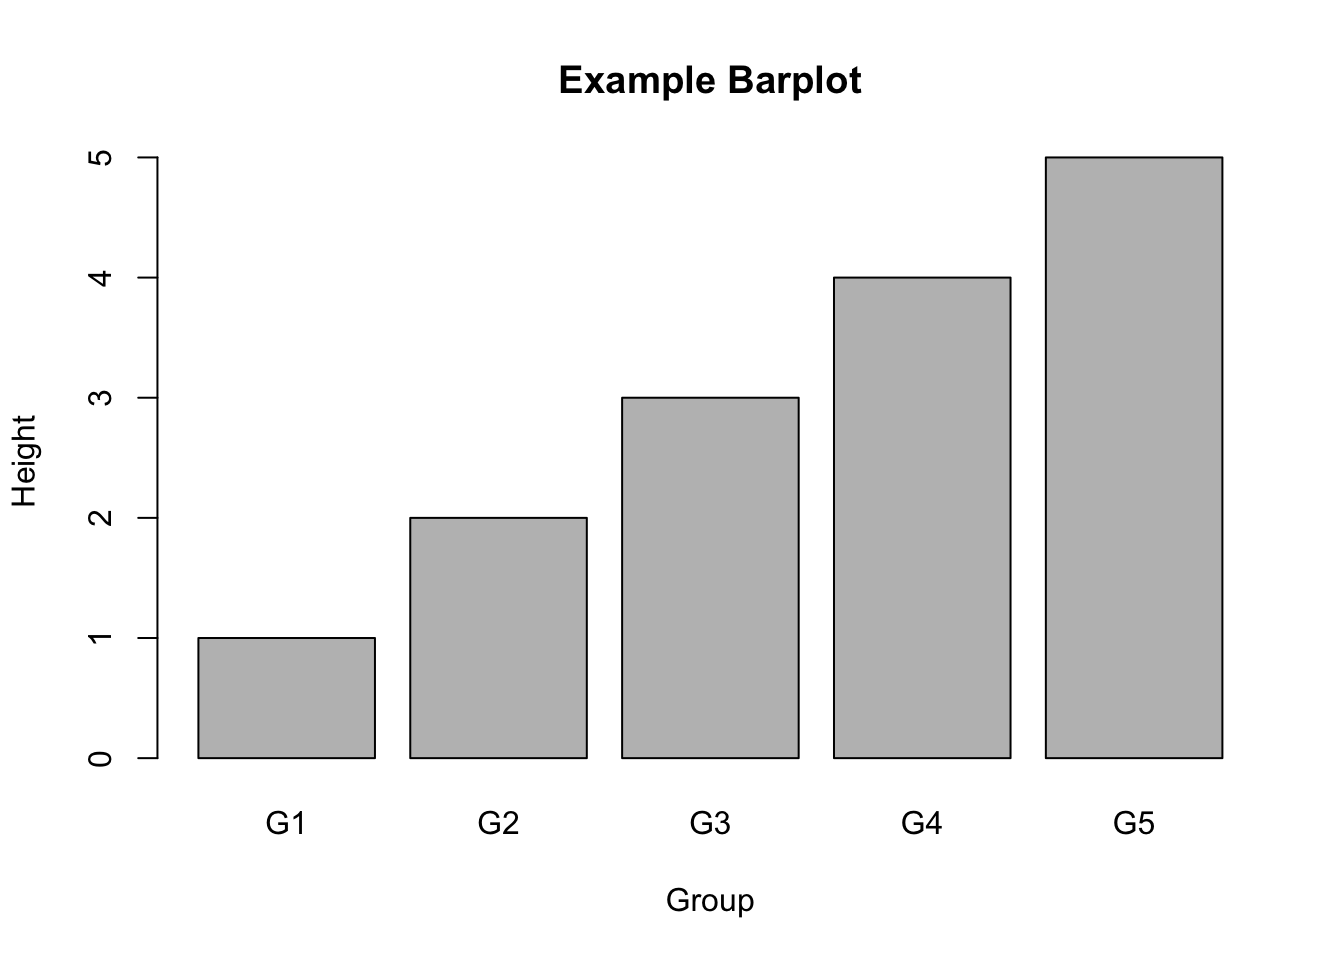
\includegraphics[width=0.4\linewidth]{Gambar/contoh barplot.png}
    \caption{Contoh visualisasi dari tinggi beberapa grup dengan menggunakan \textit{bar plot}}
    \label{fig:contoh barplot}
\end{figure}

\textit{Bar plot} merupakan teknik visualisasi data yang menggunakan batang vertikal atau horizontal untuk menunjukkan nilai-nilai dari data. Visualisasi ini berguna untuk menunjukkan pengukuran statistik sebuah data secara terpisah. \textit{Bar Plot} memiliki elemen utama yaitu sumbu \textit{x} dan sumbu \textit{y}. Gambar~\ref{fig:contoh barplot}~\cite{Phillips} merupakan contoh penggunaan \textit{bar plot} untuk memvisualisasikan data di mana pada contoh ini sumbu \textit{x} nya menunjukkan grup yang dimiliki data sedangkan sumbu \textit{y} nya menunjukkan tinggi dari masing-masing grup.